\section{Introduction}
\label{sec:introduction}

Graphics processing units (GPUs) are becoming powerful many-core compute
devices.
For example, NVIDIA GPUs integrate more than $1,500$ processing cores on
a single chip and the peak double-precision performance exceeds 1
TFLOPS while sustaining thermal design power (TDP) in the same order of
magnitude as traditional multicore CPUs~\cite{NVIDIA_Kepler}. 
This rapid growth of GPUs is due to recent advances in the
programming model, often referred to as general-purpose computing on
GPUs (GPGPU).
Data-parallel and compute-intensive applications receive significant
performance benefits using GPGPU.
Currently a main application of GPGPU is supercomputing~\cite{TOP500}
but there are more and more emerging applications in different fields.
Examples include plasma control~\cite{Kato_ICCPS13}, autonomous
driving~\cite{McNaughton_ICRA11}, software routing~\cite{Han_SIGCOMM10},
encrypted networking~\cite{Jang_NSDI11}, and storage
management~\cite{Bhatotia_FAST12, Gharaibeh_HPDC10, Kato_ATC12,
Sun_SYSTOR12}.
This broad range of applications raises the need of further developing
GPU technology to support scalability of emerging data-parallel and
compute-intensive applications.

\begin{figure}[!t]
 \centering
 \subfigure[Host to Device]{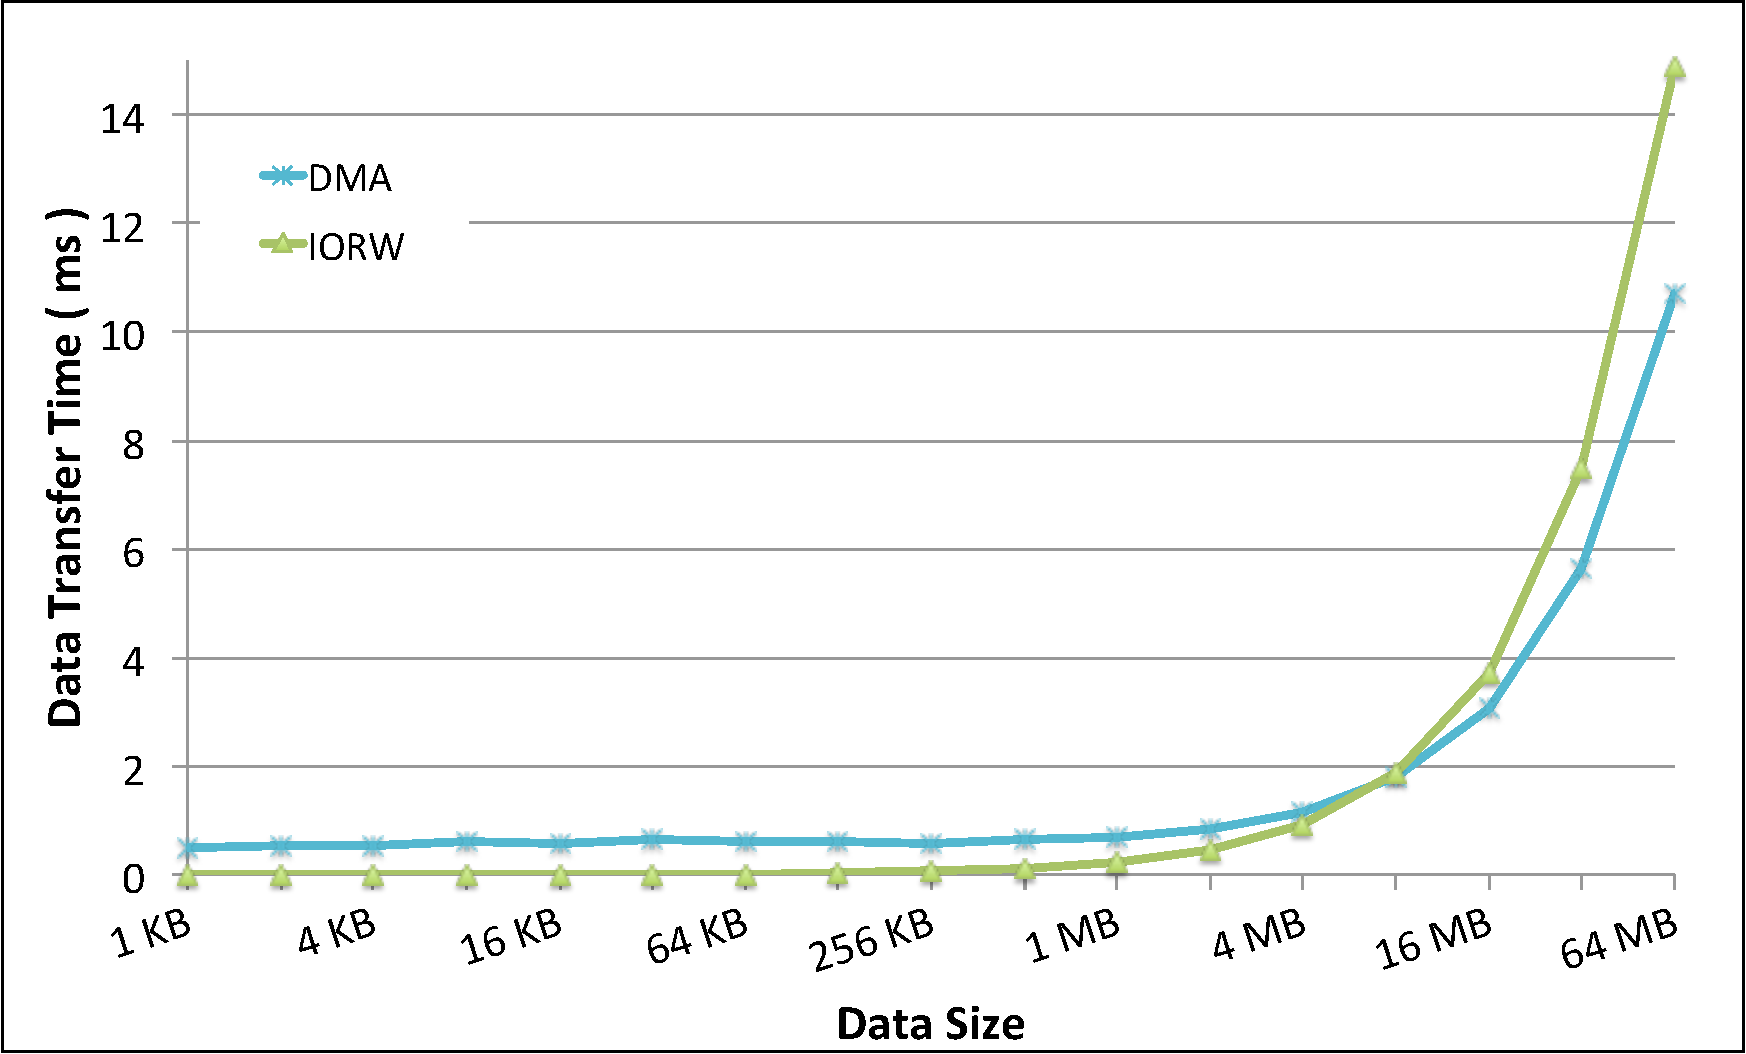
\includegraphics[width=0.34\textwidth]{figure/Graph/forIntro_HtoD.pdf}}\\
 \subfigure[Device to Host]{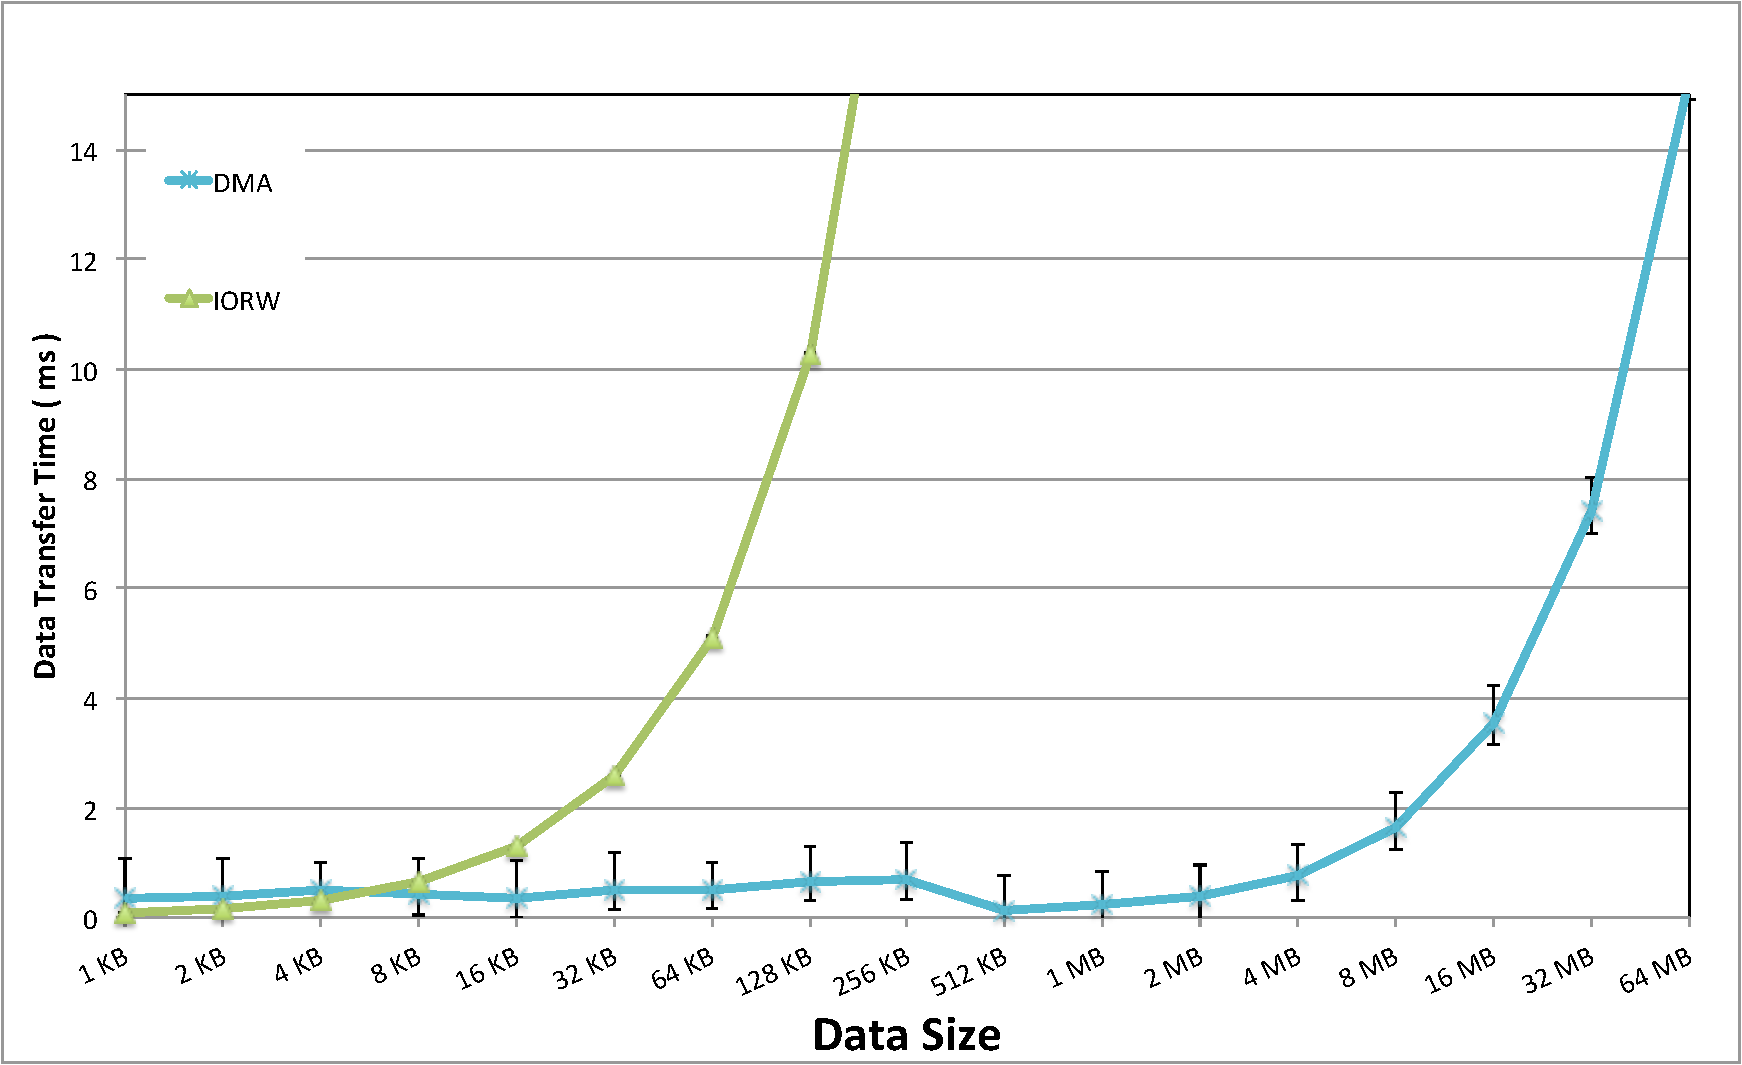
\includegraphics[width=0.34\textwidth]{figure/Graph/forIntro_DtoH.pdf}}
 \caption{Performance of DMA and I/O read/write for the NVIDIA GPU.}
 \label{fig:intro_data_transfer}
\end{figure}

One of the greatest challenges of GPU computing is to integrate
real-time systems.
So far the real-time systems community has addressed resource management
issues of GPUs~\cite{Basaran_ECRTS12, Elliott_RTS12, Elliott_ECRTS12,
Kato_ATC11, Kato_RTAS11, Kato_RTSS11}.
The main contribution of these work is the scheduling of compute
kernels and data transfers associated with the GPU.
On the other hand, the basic performance and latency issues of GPUs are
not well explored in the literature.
Given that compute kernels are offloaded to the GPU, their performance
and latency are more dominated by compiler and hardware technology.
However, an optimization of data transfers must be complemented by system
software due to constraints of PCIe devices~\cite{Kato_ATC12}.
Data transfers are also interfered by compelling workload on the CPU,
while compute kernels are protected within the GPU.
These data transfer issues must be well understood and addressed in
order to build predictable soft real-time, if not hard real-time,
systems augmented with GPUs.

Data transfer issues are particularly important for low-latency GPU
computing.
Kato~\textit{et. al.} demonstrated that the data transfer is a dominant
property for GPU-accelerated plasma control systems~\cite{Kato_ICCPS13}.
This is a specific application where data must be transferred between the
sensor/actuator devices and the GPU at a high-rate but is a good example
presenting the impact of data transfers in GPU computing.
Since emerging applications augmented with GPUs may demand a similar
performance requirement, a more general study on the GPU data transfer
is desired.

Figure~\ref{fig:intro_data_transfer} illustrates the average data
transfer times of hardware-based direct memory access (DMA) and
memory-mapped I/O read and write access performed on an NVIDIA GeForce
GTX~480 graphics card using an open-source Linux
driver~\cite{Kato_ATC12}.
Apparently the performance characteristics are not identical between the
host-to-device and the device-to-host directions.
A very elementary issue of this performance difference has been
discussed~\cite{Kato_ATC12}, but there is no clear conclusion on what
methods can optimize the data transfer performance, what different
methods are available, and what is their implication for real-time
systems.
Currently we pray that the black-box data transfer methods provided by
vendors proprietary software are well optimized, because the hardware
details of GPUs are not disclosed to the public.
However, real-time systems must build on predictable disciplines.
A better understanding of the data transfer performance for the GPU is
an essential piece of work to facilitate research on GPU-accelerated
heterogeneous real-time systems.

\textbf{Contribution:}
This paper explores data transfer methods for GPU computing and
provides their detailed empirical comparison.
We unveil several data transfer methods for the GPU in addition to
well-known DMA and I/O read and write approaches.
The advantage and disadvantage of these methods are also discussed.
The contribution of this paper provides an insight of how to design and
implement optimized data transfer methods especially in the context of
real-time systems.
We believe that this is a useful contribution to advance real-time
technology with GPUs and emerging heterogeneous compute devices.

\textbf{Organization:}
The rest of this paper is organized as follows.
Section~\ref{sec:assumption} presents the assumption and terminology
behind this paper.
Section~\ref{sec:data_transfer_methods} provides an open investigation
of data transfer methods for GPU computing.
Section~\ref{sec:empirical_comparison} compares the performances of the
investigated data transfer methods in the context of real-time systems.
Related work are discussed in Section~\ref{sec:related_work}.
We provide our concluding remarks in Section~\ref{sec:conclusion}.
